%%
% Report: First Assignment - Business Process Prediction, Simulation, and Optimization
% Built on the TUM Overleaf template (tumarticle class, files in tum/).
% Tables in tables/ and figures in figures/ are generated from the project repository
% (python -m src.report_assets).
%%

\PassOptionsToPackage{section}{placeins} % = \usepackage[section]{placeins}; the class loads placeins itself
\documentclass[
  english,        % define the document language (english, german)
  font=times,     % define main text font (helvet, times, palatino, libertine)
  twocolumn,      % use onecolumn or twocolumn layout
]{tumarticle}

\usepackage{cite}

% Add packages here:
\usepackage{booktabs}
\usepackage{makecell}
\usepackage{array}
\usepackage{graphicx}
\usepackage{caption}
\usepackage{float}
\usepackage{flafter} % a table or figure never appears before the place where it is written
% every table and figure stays in its own subsection (placeins: barrier before each subsection)
\let\oldsubsection\subsection
\renewcommand{\subsection}{\FloatBarrier\oldsubsection}

% footnote for a package / tool, same style as in the template
\newcommand{\fn}[2]{\footnote{\tiny #1: \url{#2}}}
% placeholders that still have to be filled in
\newcommand{\todo}[1]{\textcolor{red}{\textbf{[#1]}}}

% article metadata
\title{First Assignment - Business Process Prediction, Simulation, and Optimization - Winter Semester 2026/2027}
\subtitle{Process and Data Science on the BPIC-17 Event Log}

\author[email=author@tum.de]{Author (add your information here)}

\date\today

\renewcommand{\dbltopfraction}{0.9} % room for Figures 1 and 2 on one page
\renewcommand{\textfraction}{0.05}
\raggedbottom % no stretched gaps between paragraphs in short columns
\newlength{\fullwidth} % page text width, also inside minipages (appendix landscape pages)
\begin{document}

\maketitle

\begin{abstract}
This report analyses the BPI Challenge 2017 event log of a Dutch bank to build a process model for simulation. We reduced the log to 16 activities representing the work of the bank and improved an Inductive Miner model step by step. The final model is sound and replays 87.6\% of test cases with a precision of 0.821, higher than all automatically discovered models. Decision mining shows that the outcome mainly depends on whether the customer returns the offer. Clustering only partly supported the use of separate models for different scenarios, so one model with decision rules remains the better choice for simulation.
\end{abstract}
%

\section{Introduction}
This report focuses on the analysis of the BPI Challenge 2017 event log \cite{vandongen2017}, which was presented by a Dutch financial institution. The dataset captures the loan application process, covering all requests submitted in 2016 and the ways of handling them until February 2017. The process owner prepared the data for the Business Process Intelligence Challenge with the aim of asking researchers to answer key business questions regarding processing times, the impact of missing documents, and how multiple offers affect the outcome\fn{BPI Challenge 2017}{https://ais.win.tue.nl/bpi/2017/challenge.html}.

The dataset tracks three main interconnected entities: Applications (A\_), Offers (O\_), and Workflow items (W\_), each representing a different aspect of the loan application lifecycle. These refer, respectively, to the credit requests submitted by customers, the loan proposals issued by the bank, and the internal processing tasks handled by employees or the system. The full event log consists of over 31,500 cases and more than 1.2 million events.

Our results are consistent with earlier analyses. Rodrigues et al.\ stated that cancellations occur ``in most of cases [\ldots] because the applicants did not give an answer to the bank'' \cite[Sec.~7]{rodrigues2017}; similarly, two of our clusters contain cases in which the customer never returns the offer, and 98\% of them are cancelled (Section~\ref{sec:clustering}). Decision mining also showed that the outcome mainly depends on whether the customer returns the offer (Section~\ref{sec:model}). Finally, none of the automatically discovered models replayed around 80\% of the cases with high precision, so we built our own process model step by step (Section~\ref{sec:model}).

\section{Approach and Results}
The following sections describes the technical setup, the initial analysis of the event log, the creation and validation of the process model, and the advanced clustering analysis. All code, parameters, and fixed random seeds are available in the public repository:
\todo{LINK: GitHub/GitLab}

\subsection{Technical Setup}
All analyses were conducted in Python\fn{Python}{https://www.python.org} 3.11.0 using Jupyter notebooks\fn{Jupyter}{https://jupyter.org}. PM4Py\fn{PM4Py}{https://pm4py.fit.fraunhofer.de} was utilized for process discovery, conformance checking, quality assessment, and BPMN model handling. Data preparation and machine learning tasks were executed using pandas\fn{pandas}{https://pandas.pydata.org}, NumPy\fn{NumPy}{https://numpy.org}, and scikit-learn\footnote{\tiny scikit-learn: \url{https://scikit-learn.org}\label{fn:sklearn}}, while Matplotlib\fn{Matplotlib}{https://matplotlib.org} was used to create the visualisations. NetworkX\fn{NetworkX}{https://networkx.org} was used to compute our cyclicity metric, and the LP solvers CVXOPT\fn{CVXOPT}{https://cvxopt.org} and PuLP\fn{PuLP}{https://coin-or.github.io/pulp} were used internally by PM4Py to compute alignments.

The final process model follows the BPMN 2.0 standard\fn{BPMN 2.0 specification (OMG)}{https://www.omg.org/spec/BPMN/2.0/} and was created and exported with PM4Py and rendered with Graphviz\fn{Graphviz}{https://graphviz.org}. The event log was divided into training (70\% of cases) and test (30\%) sets using a fixed random seed (42). All models were discovered using the training data and evaluated on the test data.

\subsection{Basic Analysis}
Table~\ref{tab:basic} summarises the required statistics of the event log, and Table~\ref{tab:additional} adds two further analyses: the variant coverage at different abstraction levels and the outcome and throughput time of the cases.

\begin{table}[!htb]
    \caption{Basic event log statistics (full log).}
    \label{tab:basic}
    \centering
    \small
    \setlength{\tabcolsep}{3pt}
    \begin{tabular}{@{}lr@{}}
\toprule
Statistic & Value \\
\midrule
Cases & 31,509 \\
Events & 1,202,267 \\
Variants & 15,930 \\
Activities & 26 \\
Case attribute labels & 4 \\
Event attribute labels & 15 \\
Case length, mean / std & 38.16 / 16.72 \\
Case length, median [range] & 35 [10, 180] \\
Duration (d), mean / std & 21.90 / 13.17 \\
Duration (min), mean / std & 31,535.43 / 18,963.69 \\
Duration (s), mean / std & 1,892,125.92 / 1,137,821.69 \\
Duration (d), median & 19.09 \\
Categorical event attr. & 9 (7 excl. identifiers) \\
Resources & 149 \\
Observation period & 2016-01-01 to 2017-02-01 \\
\bottomrule
\end{tabular}

\end{table}

The result clearly shows us how large and highly variable the event log is. Each case contains 38 events on average, and the 31,509 cases follow 15,930 different variants. The ten most frequent variants cover only 15.3\% of the cases, which leads us to the conclusion that a process model discovered from the full log would be very complex and difficult to interpret.

\begin{table}[!htb]
    \caption{Additional statistics: (a) number of variants and share of cases covered by the most frequent variants; (b) case outcome and case duration.}
    \label{tab:additional}
    \centering
    \footnotesize
    \setlength{\tabcolsep}{1.5pt}
    \begin{tabular}{@{}lrrrr@{}}
\toprule
\multicolumn{5}{@{}l}{\textbf{(a) Variant coverage by abstraction level}} \\
Abstraction & Events & Variants & \makecell[r]{Top-10\\var.\ (\%)} & \makecell[r]{Var.\ for\\80\,\%} \\
\midrule
Full log & 1,202,267 & 15,930 & 15.3 & 9,629 \\
Complete events & 475,306 & 5,623 & 31.2 & 610 \\
A\_ and O\_ events & 433,444 & 2,630 & 56.7 & 65 \\
16 activities & 361,008 & 2,912 & 48.5 & 100 \\
\midrule
\multicolumn{5}{@{}l}{\textbf{(b) Case outcome and throughput time}} \\
Outcome & Cases & \makecell[r]{\% of\\cases} & \makecell[r]{Median\\(days)} & \makecell[r]{Mean / std\\(days)} \\
\midrule
Pending & 17,228 & 54.7 & 14.8 & 18.1 / 11.7 \\
Cancelled & 10,431 & 33.1 & 31.6 & 29.9 / 12.4 \\
Denied & 3,752 & 11.9 & 14.1 & 16.8 / 10.8 \\
None (open) & 98 & 0.3 & 27.0 & 28.7 / 21.0 \\
\bottomrule
\end{tabular}

\end{table}

Table~\ref{tab:additional}a demonstrates the strength of variability dependence on the abstraction level. While 9,629 variants are needed to cover 80\% of the cases in the full log, only 610, 65 or 100 on the three reduced levels. This explains the level of detail chosen for the process model in Section~\ref{sec:model}.

Table~\ref{tab:additional}b shows that 54.7\% of the applications end with an approved loan, 33.1\% are cancelled, and 11.9\% are denied. Cancelled cases take the longest, with a median of 31.6 days. This suggests that many applications are cancelled automatically when the customer does not respond. The 98 open cases without an outcome were removed before further analysis.

\subsection{Process Model}
\label{sec:model}
\paragraph{Preprocessing:}
We modelled the process at the level of the work performed by the bank. Most A\_ events only record status changes and have a corresponding W\_ event, which describes the same step from the employees' side. We therefore replaced A\_Concept and A\_Accepted with W\_Complete application, A\_Complete with W\_Call after offers, A\_Validating with W\_Validate application, and A\_Incomplete with W\_Call incomplete files. A\_Submitted was kept as a customer action, since W\_Handle leads was not started in most online applications. The lifecycle transitions of W\_ events (schedule, start, suspend, resume) create many short loops. To avoid this, each work item was represented by a single event, and work items that were never started were removed.

Other decisions were to remove O\_Created, as it is only a system confirmation of O\_Create Offer, to merge the two O\_Sent activities, and to exclude three rare W\_ activities (each occurring in no more than 1\% of cases). The resulting log comprises 16 activities and requires only 100 variants to cover 80\% of cases (Table~\ref{tab:additional}a). Open cases were removed, and the closed cases were split into a training set (70\%) and a test set (30\%). Based on the variant analysis, models were trained on the variants that cover 90\% of the training cases and evaluated on all test cases.

\paragraph{Process discovery:}
We applied two types of models, where one is the Inductive Miner \cite{leemans2014} with noise thresholds of 0.0, 0.2, and 0.4, and the other is the Heuristics Miner \cite{weijters2006} (the resulting models are shown in Appendix~\ref{app:discovered}). Table~\ref{tab:discovery} shows the quality metrics calculated with PM4Py and two simplicity metrics implemented by us based on Carmona et al.\ \cite{carmona2018}: model size (number of places and transitions) and control-flow complexity (CFC). None of the discovered models reaches the target of about 80\% fitting cases with high precision. Without noise filtering, the Inductive Miner replays 99.7\% of cases but has a low precision of 0.44. With a threshold of 0.4, precision improves to 0.78, but only 31.9\% of cases can be replayed. The Heuristics Miner model is unsound and replays no test case completely, so its precision value is not reliable.

\begin{table}[!htb]
    \caption{Quality of the discovered models on the log with 16 activities (test set). Fitting cases, average fitness and precision are alignment-based; Simpl.\ (arc) is the PM4Py simplicity; Size and CFC are our own simplicity metrics. $^{*}$\,Token-based replay, since alignments are not possible for the unsound HM model.}
    \label{tab:discovery}
    \centering
    \footnotesize
    \setlength{\tabcolsep}{2pt}
    \begin{tabular}{@{}lcrrrrrrr@{}}
\toprule
Model & Sound & \makecell[r]{Fit.\\\%} & \makecell[r]{Avg\\fit.} & Prec. & Gen. & \makecell[r]{Simpl.\\(arc)} & Size & CFC \\
\midrule
IM 0.0 & yes & 99.7 & 1.000 & 0.438 & 0.966 & 0.660 & 97 & 45 \\
IM 0.2 & yes & 64.9 & 0.965 & 0.713 & 0.981 & 0.684 & 65 & 29 \\
IM 0.4 & yes & 31.9 & 0.920 & 0.776 & 0.981 & 0.700 & 56 & 22 \\
HM & no & 0.0$^{*}$ & 0.721$^{*}$ & 1.000$^{*}$ & 0.940$^{*}$ & 0.596 & 62 & 34 \\
\bottomrule
\end{tabular}

\end{table}

\paragraph{Iterative refinement:}
IM 0.2 performed the best balance between fitness and precision among all models. Additionally, it already treats A\_Submitted as optional unlike to IM 0.4. We then improved the model in four steps, using the discovered models, statistics from Section~2.2, previous reports, and domain knowledge (Table~\ref{tab:versions}).

Although the Inductive Miner placed W\_Validate application, O\_Returned, and W\_Call incomplete files in parallel, the data show us that these steps follow the order: O\_Returned after the validation process. Validation and calls never overlap, and two calls for missing documents are never made without another validation in between. For this reason, we replaced the parallel block with a sequence and a validation loop (v01). This increased precision from 0.713 to 0.803, while fitness decreased slightly. We can conclude that the parallelism was caused by the algorithm rather than actual parallel work. We kept separate loops for creating and sending offers because several offers are usually created first and sent afterwards. Combining both activities into one loop reduced fitness and precision.

The next step addressed the largest group of non-fitting cases of the model. About 19\% of the cases contain later offers, which are mostly created during W\_Call after offers or W\_Call incomplete files and then followed by validation instead of a new call. In v02, a separate block was added for later offers after both calls. This change substantially increased the share of fitting cases from 63.2\% to 72.7\%.

All previous models also allowed A\_Denied after an application had been approved or cancelled. In v03, we changed the outcome to an exclusive choice between approval, denial, and cancellation. This increased the share of fitting cases to 82.0\% and precision to 0.821.

In the final version (v04), we made W\_Complete application optional because it is not started in every case. However, it is skipped only for online applications, so we allowed this only for them. Allowing it in all cases lowered precision. The change increased the share of fitting cases to 87.6\%, while precision stayed at 0.821.

Generalization remained stable at 0.97--0.98 after the first refinement, indicating that the changes did not lead to overfitting.

\begin{table}[!htb]
    \caption{Iterative refinement of the process model (test set). v00 is IM 0.2; each version changes the previous one. Fitting cases, precision and generalization are alignment-based.}
    \label{tab:versions}
    \centering
    \footnotesize
    \setlength{\tabcolsep}{1.8pt}
    \begin{tabular}{@{}llrrrrr@{}}
\toprule
Ver. & Change & Fit.\ \% & Prec. & Gen. & Size & CFC \\
\midrule
v00 & IM 0.2 (baseline) & 64.9 & 0.713 & 0.981 & 65 & 29 \\
v01 & sequential validation & 63.2 & 0.803 & 0.982 & 58 & 26 \\
v02 & later-offer block & 72.7 & 0.801 & 0.980 & 84 & 33 \\
v03 & one outcome (XOR) & 82.0 & 0.821 & 0.973 & 85 & 34 \\
v04 & W\_Complete appl.\ optional & 87.6 & 0.821 & 0.973 & 90 & 36 \\
\bottomrule
\end{tabular}

\end{table}

\begin{figure*}[t]
    \centering
    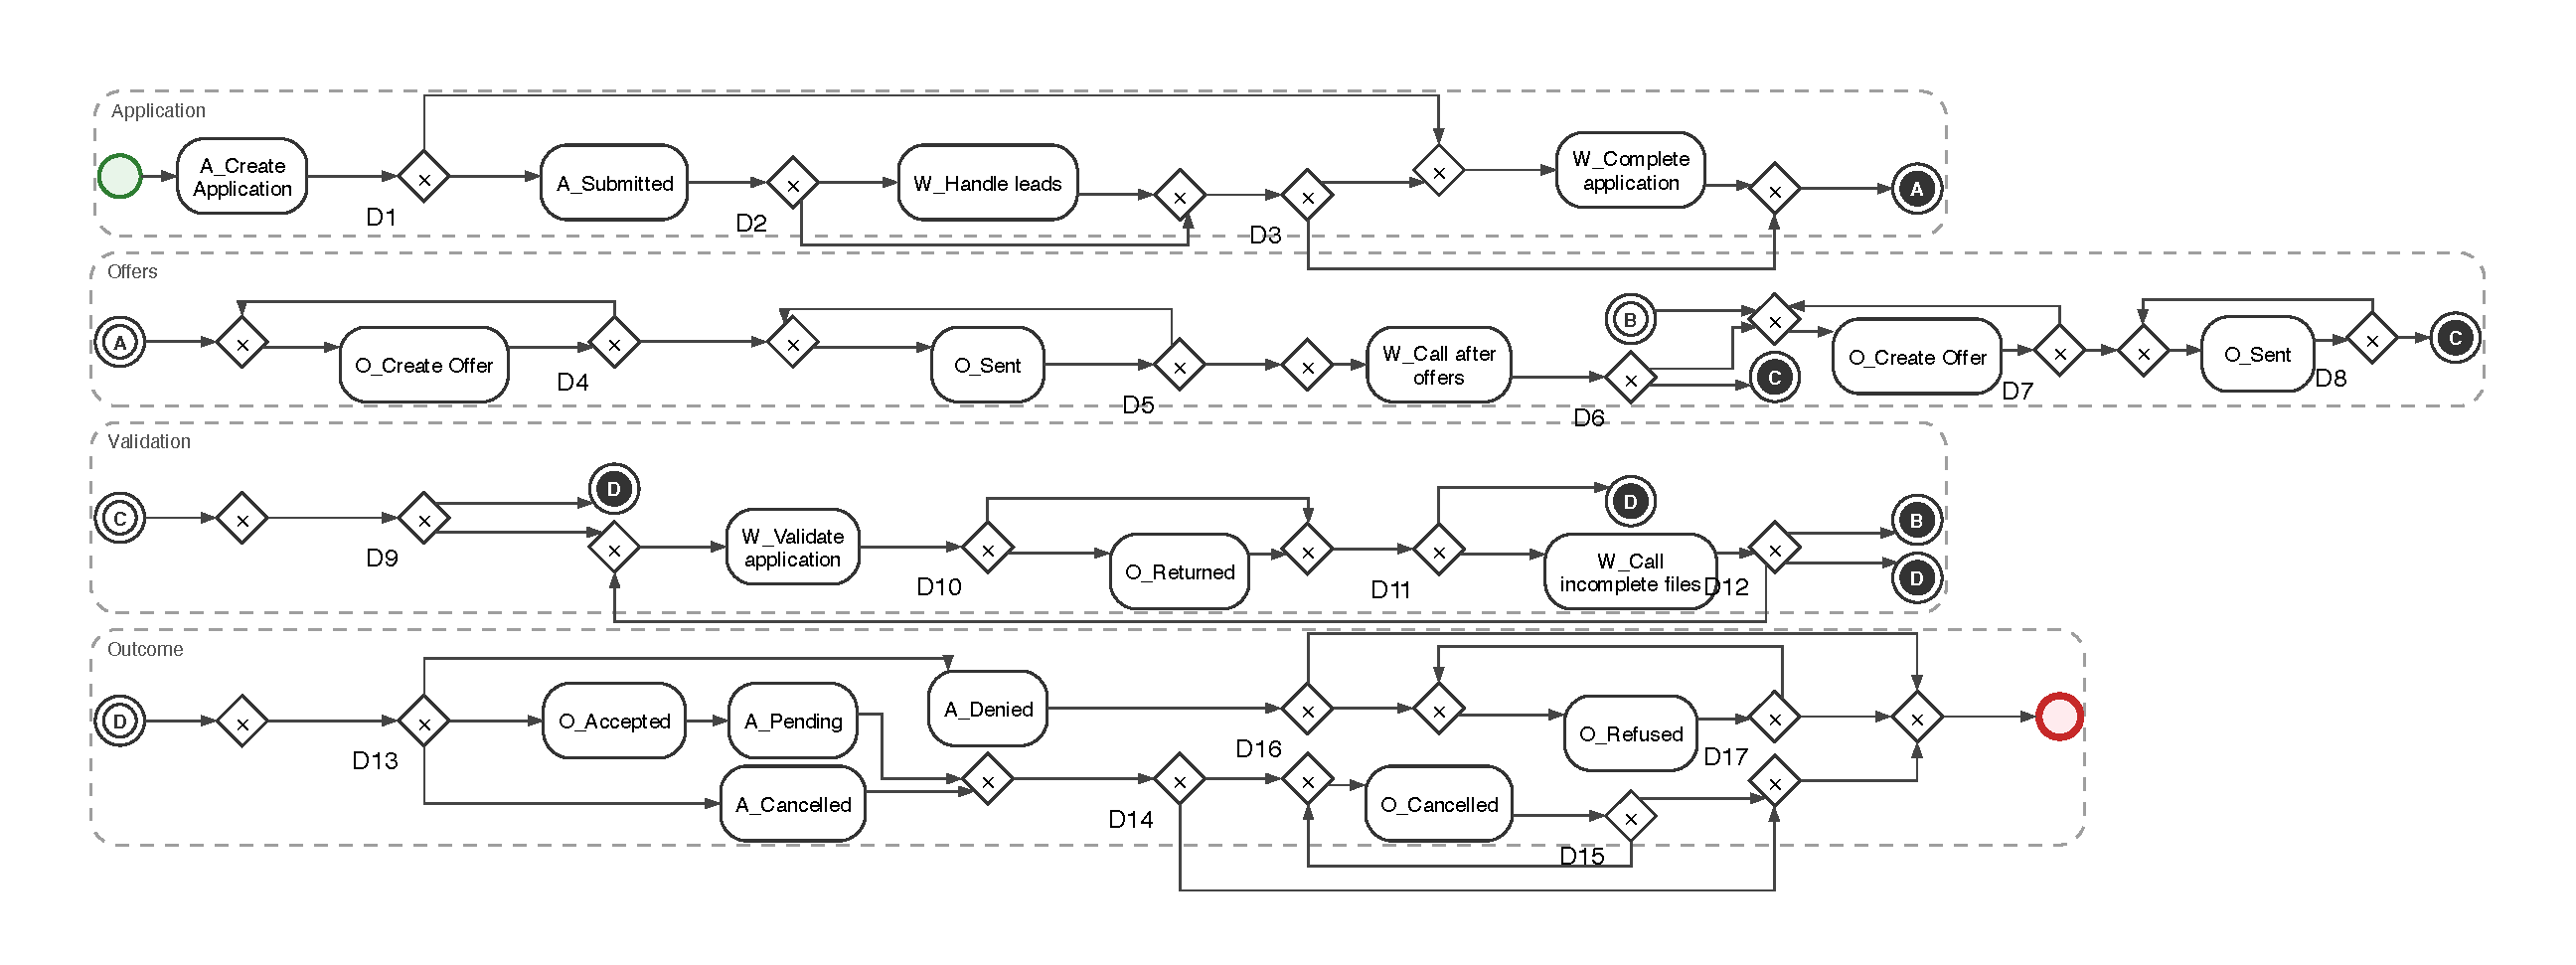
\includegraphics[width=\textwidth,height=0.42\textheight,keepaspectratio]{figures/final_model.pdf}
    \caption{Final process model (v04) as BPMN 2.0, split into four blocks; the circles with letters are link events that connect the rows. Labels D1--D17 mark the XOR gateways analysed in the decision mining (Table~\ref{tab:decisions}, Figure~\ref{fig:decisions} in Appendix~\ref{app:discovered}).}
    \label{fig:bpmn}
\end{figure*}

The final model (Figure~\ref{fig:bpmn}) is sound and replays 87.6\% of the test cases with a precision of 0.821 and a generalization of 0.973. It has the highest precision and higher fitness than all discovered models except IM 0.0. The price is a larger model than IM 0.2 and IM 0.4 (size 90 compared to 65 and 56).

We focused on prioritizing precision and soundness over simplicity, because the model serves as the base model for a simulation. A sound model cannot deadlock, and a precise model does not generate behaviour that never occurs in reality. We did not aim for 100\% fitness because modelling rare cases would make the model unnecessarily complex, with too many additional paths and loops. The model also has some limitations. Each work item is recorded as a single event. This means that pauses and resumptions are only reflected in its duration. Most remaining non-fitting cases are caused by three situations: O\_Returned directly after W\_Call incomplete files, O\_Cancelled during the process when an offer is replaced, and alternating creation and sending of offers. Finally, the model cannot show which offer was accepted and which were cancelled, as it presents applications rather than individual offers.

\paragraph{Decision mining:}
Following de Leoni and van der Aalst \cite{deleoni2013}, we used alignments to identify the chosen branch at each XOR gateway. For each decision, we used case attributes and historical information, such as the number of offers and missing documents. We trained decision trees (depth 3) on the training set and compared their accuracy and macro-F1 with a baseline that always predicts the most frequent branch. Selected and CreditScore were excluded because they show the final outcome. For the same reason, we did not use the duration and end type of W\_ work items.

\begin{table}[!htb]
    \caption{Decision mining at the XOR gateways D1--D17 of the final model (test set): majority baseline vs.\ decision tree (CART, depth 3). Expl.\ = explained by the tree.}
    \label{tab:decisions}
    \centering
    \footnotesize
    \setlength{\tabcolsep}{2.5pt}
    \begin{tabular}{@{}llccl@{}}
\toprule
ID & Decision & \makecell{Accuracy\\base / tree} & \makecell{Macro-F1\\base / tree} & Expl. \\
\midrule
D1 & online submission & 0.65 / 0.83 & 0.39 / 0.78 & yes \\
D2 & W\_Handle leads (online) & 0.82 / 0.82 & 0.45 / 0.45 & no \\
D3 & W\_Complete appl.\ (online) & 0.90 / 0.90 & 0.47 / 0.47 & no \\
D4 & create one more offer & 0.89 / 0.89 & 0.47 / 0.47 & no \\
D5 & send one more offer & 0.92 / 0.92 & 0.48 / 0.58 & partly \\
D6 & later offer or continue & 0.86 / 0.86 & 0.46 / 0.46 & no \\
D7 & one more later offer & 0.94 / 0.94 & 0.48 / 0.48 & no \\
D8 & send one more later offer & 0.85 / 0.85 & 0.46 / 0.51 & partly \\
D9 & validation or outcome & 0.71 / 0.71 & 0.41 / 0.41 & no \\
D10 & O\_Returned in validation & 0.56 / 0.94 & 0.36 / 0.94 & yes \\
D11 & after validation & 0.59 / 0.64 & 0.37 / 0.62 & yes \\
D12 & after missing documents & 0.67 / 0.67 & 0.27 / 0.27 & no \\
D13 & outcome & 0.56 / 0.87 & 0.24 / 0.77 & yes \\
D14 & cancel open offers & 0.53 / 1.00 & 0.34 / 1.00 & yes \\
D15 & cancel one more offer & 0.79 / 1.00 & 0.44 / 1.00 & yes \\
D16 & refuse open offers & 0.99 / 0.99 & 0.50 / 0.50 & no \\
D17 & refuse one more offer & 0.80 / 1.00 & 0.44 / 1.00 & yes \\
\bottomrule
\end{tabular}

\end{table}

The results (Table~\ref{tab:decisions}, Figure~\ref{fig:decisions}) show that some decisions depend on case attributes or previous events. Limit raise applications are never submitted online (D1). The steps after validation depend on whether the offer was returned and whether documents were missing before (D10, D11). The final outcome (D13) mainly depends on whether the customer returns the offer: without O\_Returned, 98\% of applications are cancelled (macro-F1: 0.24 $\rightarrow$ 0.77). Other decisions follow fixed system rules, such as sending all created offers and cancelling or refusing offers while other offers remain open (D5, D8, D14, D15, D17).

Eight decisions could not be explained by the available data (D2, D3, D4, D6, D7, D9, D12, D16). In particular, the decision to proceed to document validation after W\_Call after offers (D9) seems to depend on customer responses, which are not recorded at that point. This is consistent with Rodrigues et al.\ \cite{rodrigues2017}, who found that most cancellations are caused by customers not responding.

For simulation, we can use learned rules for explainable decisions, fixed rules for system decisions, and probabilities for the remaining ones. A timer could be used for D9 to represent customer response delays.

\subsection{Advanced Analysis -- Clustering}
\label{sec:clustering}
\textbf{Hypothesis.} Our main goals are to determine whether the process consists of several simpler behavioural scenarios and whether models discovered per scenario are more precise and simpler than one global model. If this is true, a simulation could combine simple scenario models instead of one complex model. The hypothesis is confirmed if the weighted cluster models improve fitting cases and precision by at least 0.05 over the global model and every cluster model is smaller. Partially confirmed if this holds for at least one cluster on its own test cases; otherwise, rejected.

\textbf{Approach.} Each case was described by six features computed from the original log: number of offers, A\_Incomplete and A\_Validating events, occurrence of A\_Submitted and O\_Returned, and the case duration. The outcome was not included. We used K-means\textsuperscript{\ref{fn:sklearn}} to group the training cases, testing values of k from 2 to 10, where k = 8 was selected based on the silhouette score. We also checked the stability of the clusters using five additional random seeds and the Adjusted Rand Index (ARI). The global and cluster models were then discovered using the same settings as in Section~\ref{sec:model} (IM 0.2, 90\% of training variants) and evaluated on the test cases. Each cluster model was compared with the global model using the same test cases.

\begin{table}[!htb]
    \caption{Cluster profiles (training cases): share of cases, mean number of offers (Off.), A\_Incomplete (Inc.) and A\_Validating (Val.) events, share with A\_Submitted (Sub.) and O\_Returned (Ret.), median duration and outcome shares. The outcome was not used for clustering.}
    \label{tab:clusters}
    \centering
    \small
    \setlength{\tabcolsep}{1.4pt}
    \begin{tabular}{@{}lrrrrrrrrrr@{}}
\toprule
Cl. & \makecell[r]{Share\\\%} & Off. & Inc. & Val. & Sub. & Ret. & \makecell[r]{Days\\(med.)} & \makecell[r]{Pend.\\\%} & \makecell[r]{Den.\\\%} & \makecell[r]{Canc.\\\%} \\
\midrule
0 & 19 & 1.2 & 0.5 & 1.4 & 0.0 & 1.0 & 12 & 84 & 13 & 3 \\
1 & 4 & 1.8 & 1.6 & 2.1 & 0.8 & 1.0 & 47 & 66 & 10 & 24 \\
2 & 28 & 1.2 & 0.6 & 1.4 & 1.0 & 1.0 & 14 & 71 & 26 & 3 \\
3 & 22 & 1.3 & 0.0 & 0.0 & 1.0 & 0.0 & 32 & 0 & 2 & 98 \\
4 & 4 & 3.7 & 1.0 & 1.6 & 0.7 & 0.9 & 23 & 72 & 12 & 16 \\
5 & 6 & 1.4 & 2.4 & 3.0 & 0.0 & 1.0 & 18 & 90 & 6 & 4 \\
6 & 8 & 1.2 & 0.0 & 0.0 & 0.0 & 0.0 & 31 & 0 & 2 & 98 \\
7 & 9 & 1.4 & 2.4 & 2.9 & 1.0 & 1.0 & 20 & 88 & 7 & 5 \\
\bottomrule
\end{tabular}

\end{table}

\textbf{Results.} The clusters suggest several behavioral scenarios (Table~\ref{tab:clusters}): fast approvals (clusters 0, 2), cases in which customers do not return the offer (3, 6; around 31 days, 98\% cancelled), repeated requests for missing documents (5, 7; 88--90\% approved), cases with around four offers (4), and long-running cases (1). Three pairs of clusters (0/2, 3/6, and 5/7) differ mainly in whether the application was submitted online. This may be because K-means tends to split cases based on binary features and could also explain the limited stability of the clustering (minimum ARI 0.677). Overall, the cluster models performed better than the global model (fitness: 0.731 vs.\ 0.649; precision: 0.726 vs.\ 0.713), since the global model on the abstraction level is already fairly precise. However, cluster 1 and 4 produced a larger model than the global one, the model of cluster 5 shows signs of overfitting, and only clusters 0 and 2 performed better on their own cases while also producing smaller models. Therefore, the hypothesis is \textbf{partially confirmed}. Together, all cluster models have a total size of 426, which is still much larger than the final model from Section~\ref{sec:model} (size 90, fitness 0.876, precision 0.821; Figure~\ref{fig:comparison}).

\begin{figure}[!htb]
    \centering
    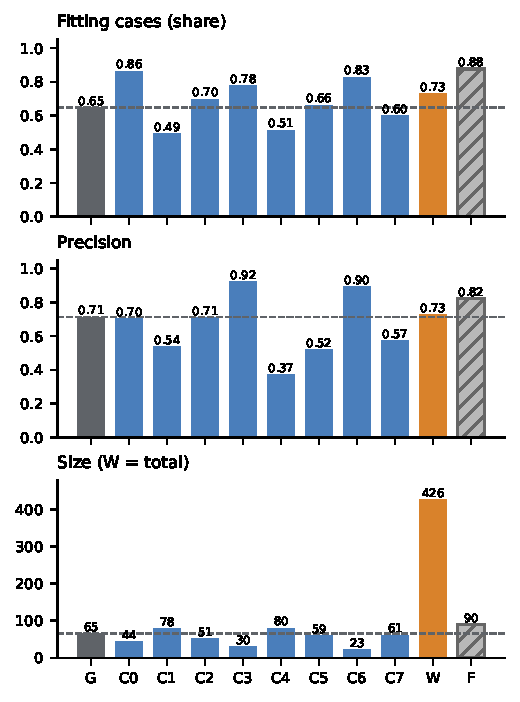
\includegraphics[width=\columnwidth]{figures/model_comparison.pdf}
    \caption{Global model (G), cluster models (C0--C7), their weighted mean (W; for size: total size of all cluster models) and the final model of Section~\ref{sec:model} (F) on the test set. The dashed line marks the global model.}
    \label{fig:comparison}
\end{figure}

\textbf{Interpretation.} Separate cluster models are not useful for simulation because the improvement is small, the clustering is unstable, and the models are much more complex. The final model with decision rules is therefore a better starting point. However, the clusters still provide useful information for the simulation. For example, cases where customers do not respond suggest using a timer of around 31 days for D9. The clusters also show different outcome rates and case durations. In addition, cases with repeated requests for missing documents are mostly approved, which is consistent with Blevi et al.\ \cite{blevi2017}.

\section*{GenAI Usage Declaration}
Claude (Anthropic) was used as a coding assistant for the analysis code and for preparing the report in LaTeX/Overleaf. Claude and ChatGPT (OpenAI) were used to structure the report and to refine formulations, and Grammarly was used to correct grammatical errors. All results and the final text were checked by the author.

%
\bibliographystyle{plain}
\bibliography{references}

\clearpage
\onecolumn
\setlength{\fullwidth}{\textwidth}
\appendix

\section{Process Models}
\label{app:discovered}
% landscape page: final model with the decision blocks (readable size)
\begin{center}
    \rotatebox{90}{\begin{minipage}{0.95\textheight}
        \centering
        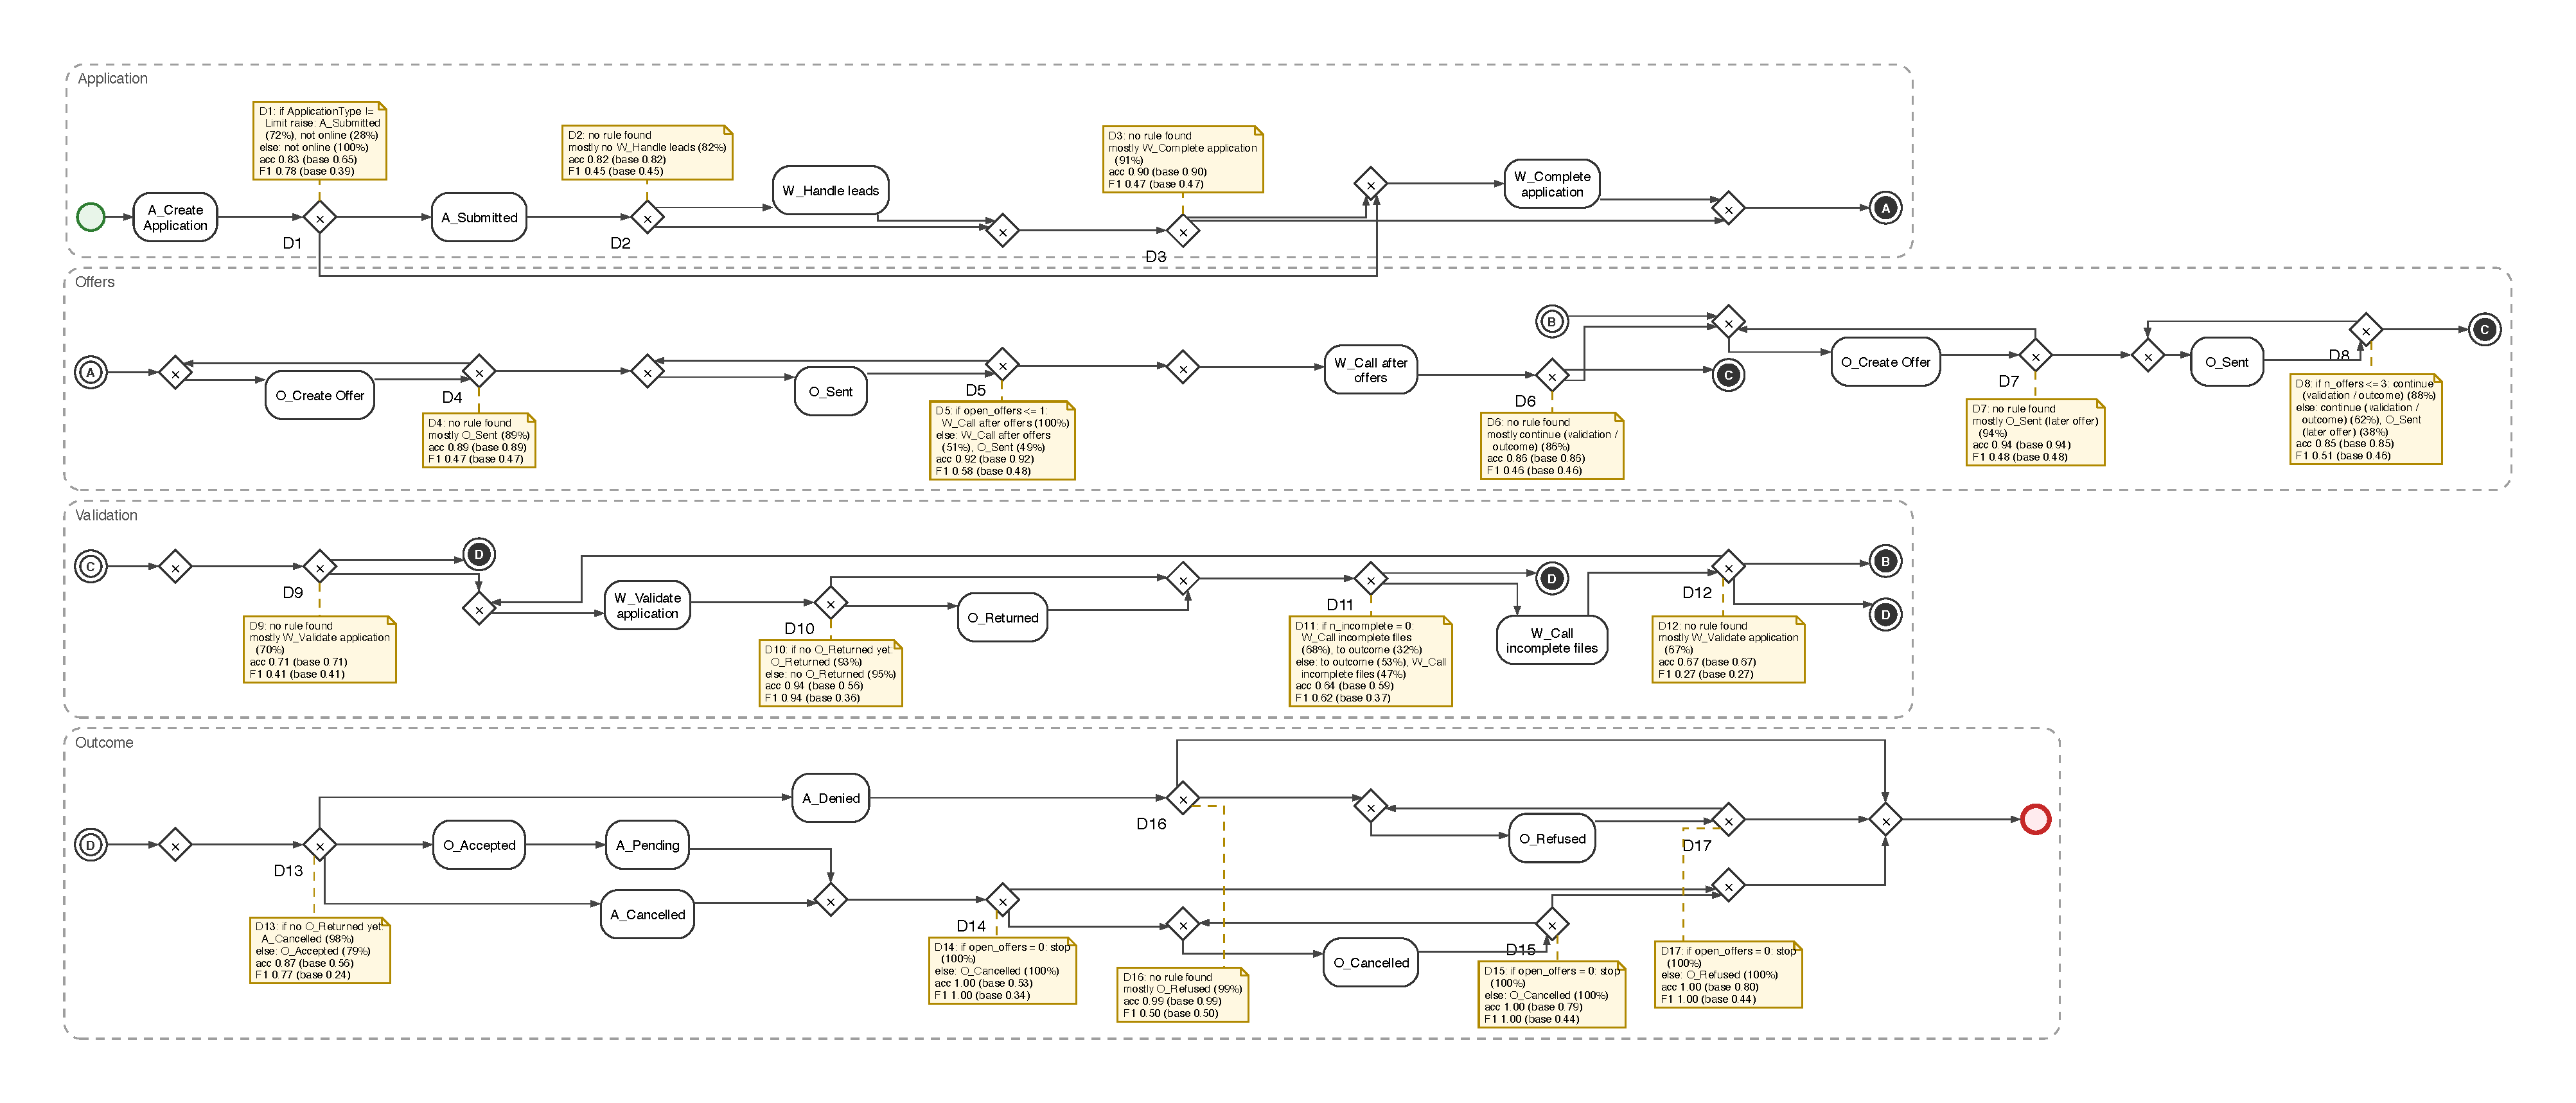
\includegraphics[width=\linewidth,height=0.85\fullwidth,keepaspectratio]{figures/final_model_decisions.pdf}
        \captionof{figure}{Final process model with a decision block at every XOR gateway (D1--D17): the main rule of the decision tree with the share of the branches, and the accuracy and macro-F1 of the tree vs.\ the majority baseline (test set).}
        \label{fig:decisions}
    \end{minipage}}
\end{center}

\clearpage
% landscape block (not a float, so it stays on the page of the section title):
% the four discovered models, rotated by 90 degrees to use the page height
\begin{center}
    \rotatebox{90}{\begin{minipage}{0.9\textheight}
        \centering
        
\includegraphics[width=\linewidth,height=0.2\fullwidth,keepaspectratio]{figures/discovered_IM_0.0.pdf}
        \captionof{figure}{Inductive Miner, noise threshold 0.0 (BPMN).}
        \label{fig:im00}
        \vspace{4pt}
        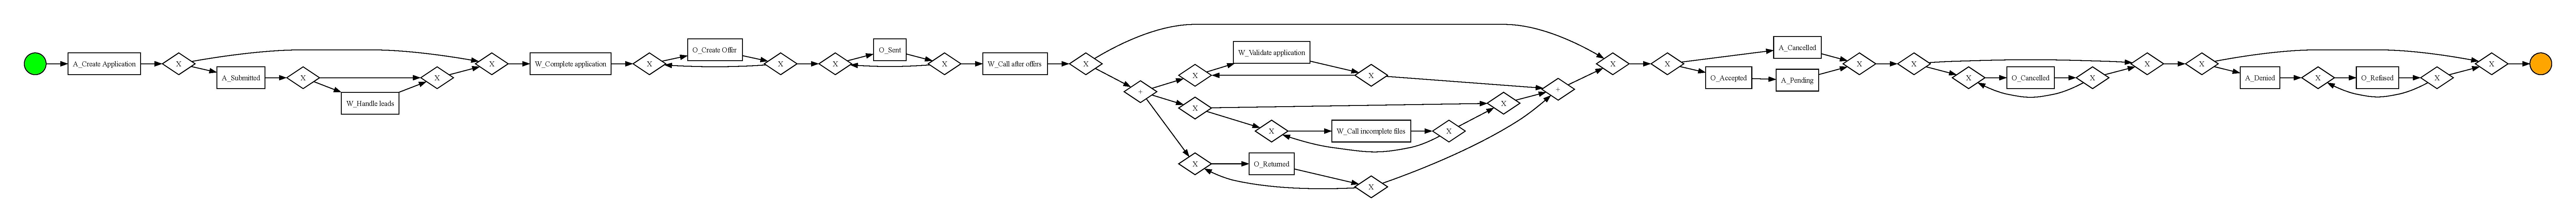
\includegraphics[width=\linewidth,height=0.2\fullwidth,keepaspectratio]{figures/discovered_IM_0.2.pdf}
        \captionof{figure}{Inductive Miner, noise threshold 0.2 (BPMN); starting point v00 of the iterative refinement.}
        \label{fig:im02}
        \vspace{4pt}
        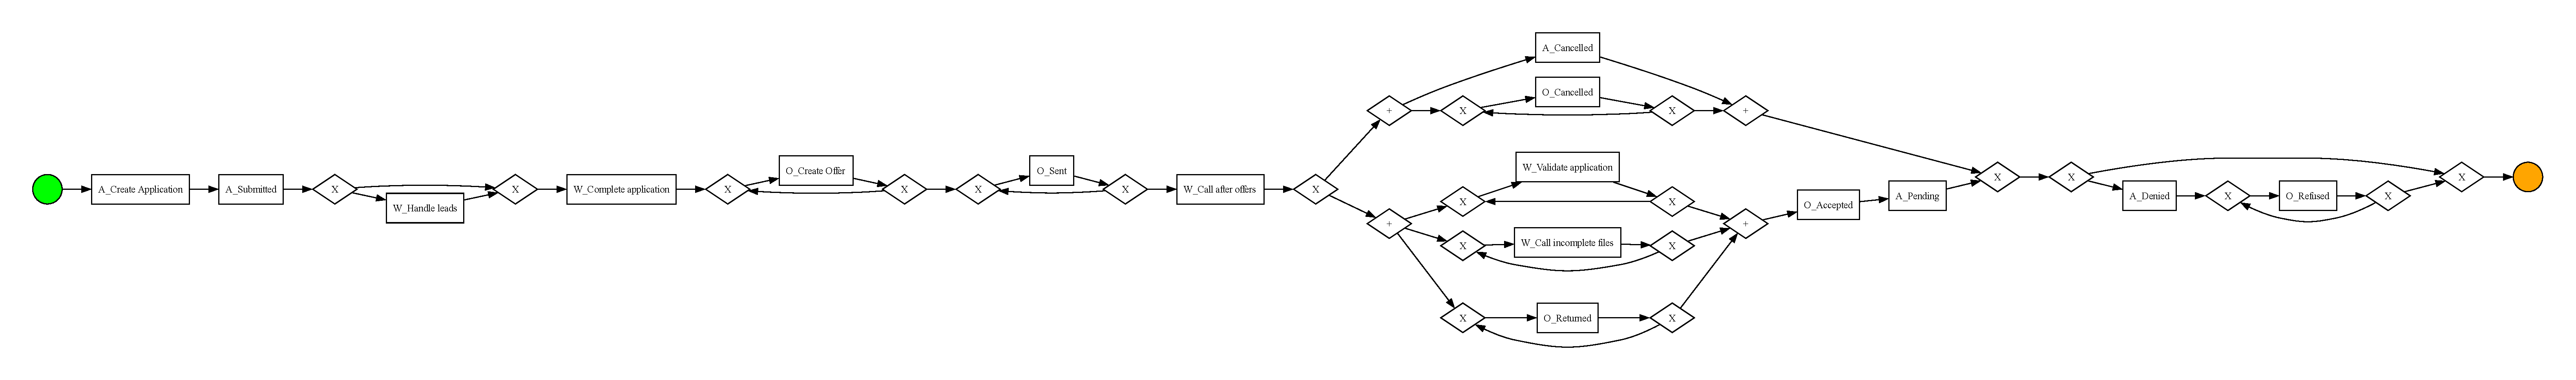
\includegraphics[width=\linewidth,height=0.2\fullwidth,keepaspectratio]{figures/discovered_IM_0.4.pdf}
        \captionof{figure}{Inductive Miner, noise threshold 0.4 (BPMN).}
        \label{fig:im04}
        \vspace{4pt}
        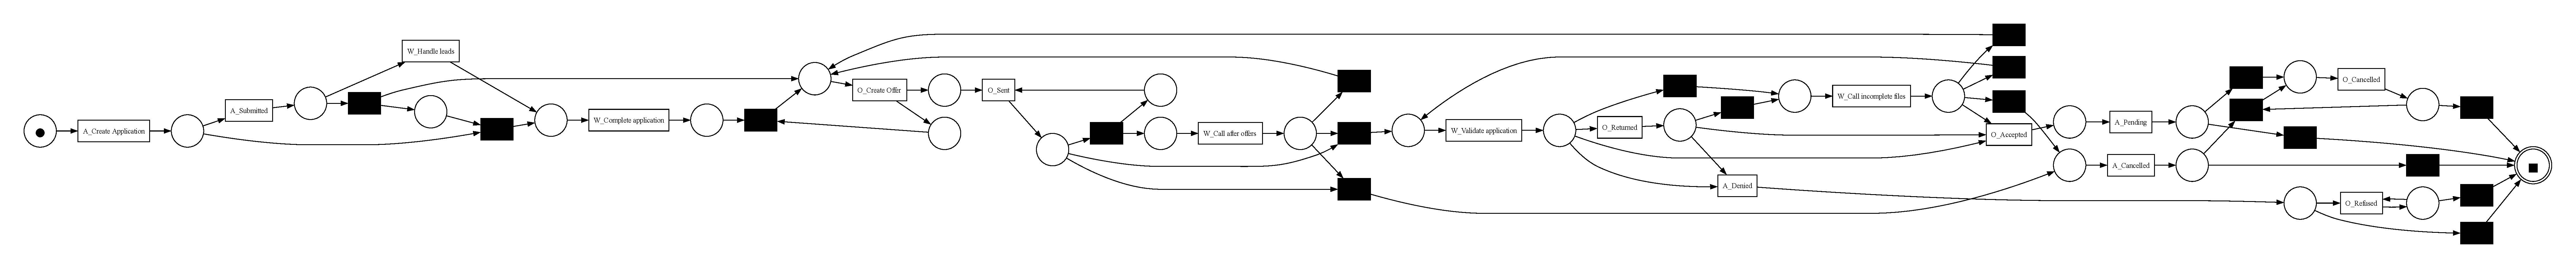
\includegraphics[width=\linewidth,height=0.2\fullwidth,keepaspectratio]{figures/discovered_HM.pdf}
        \captionof{figure}{Heuristics Miner (Petri net; not sound).}
        \label{fig:hm}
    \end{minipage}}
\end{center}

\clearpage
\section{Clustering}
\label{app:clustering}
\begin{figure}[H]
    \centering
    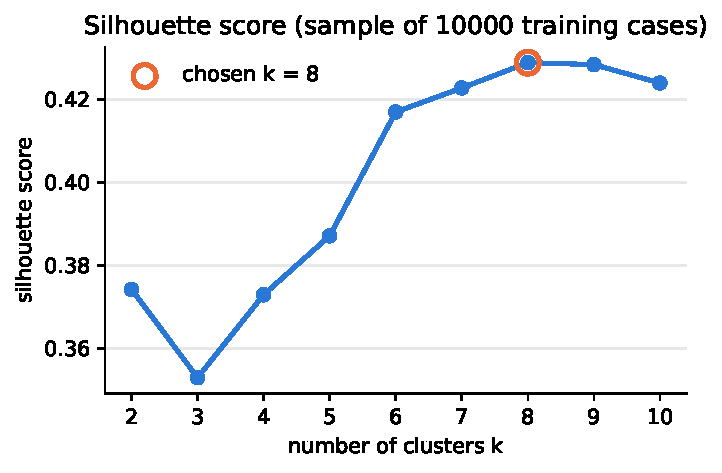
\includegraphics[width=0.5\textwidth]{figures/silhouette.pdf}
    \caption{Silhouette score for k = 2, \ldots, 10 (random sample of training cases); k = 8 was selected.}
    \label{fig:silhouette}
\end{figure}

\begin{table}[H]
    \caption{Stability of the clustering: Adjusted Rand Index between K-means runs with different random seeds (* = main run, seed 42).}
    \label{tab:ari}
    \centering
    \small
    \begin{tabular}{@{}lrrrrrr@{}}
\toprule
Seed & 42* & 1 & 2 & 3 & 4 & 5 \\
\midrule
42* & 1.000 & 0.677 & 0.996 & 0.788 & 0.764 & 0.762 \\
1 & 0.677 & 1.000 & 0.677 & 0.815 & 0.818 & 0.819 \\
2 & 0.996 & 0.677 & 1.000 & 0.787 & 0.762 & 0.759 \\
3 & 0.788 & 0.815 & 0.787 & 1.000 & 0.957 & 0.952 \\
4 & 0.764 & 0.818 & 0.762 & 0.957 & 1.000 & 0.995 \\
5 & 0.762 & 0.819 & 0.759 & 0.952 & 0.995 & 1.000 \\
\bottomrule
\end{tabular}

\end{table}

\end{document}
